\documentclass{report}
\usepackage[utf8]{inputenc}
\usepackage[top=1cm, bottom=2cm, left=2cm, right=2cm]{geometry}
\usepackage[francais]{babel}
\usepackage[T1]{fontenc}
\usepackage{graphicx}
\usepackage{subcaption}
\usepackage{listings}
\usepackage{hyperref}
\usepackage{wrapfig}

\title{Rapport}
\author{François PIAT}
\date{WEEK 5 }

\begin{document}

\maketitle

\chapter*{Profiling}

\paragraph{Problèmes}

- Le profiling n'a pas révélé d'informations pertinentes lorsque TBB est activé, puisqu'il ne considérait pas les informations passées dans les différents threads. (cf rapport-week4 , rubrique profiling/problèmes). \newline
	$\Longrightarrow$ \textit{il a fallu appliquer la commande suivante lors de l'exécution du test de callgrind pour créer un fichier dédié à chaque thread.}
	\begin{lstlisting} 
	--separate-threads=yes 
	\end{lstlisting} 
	Cette commande a été trouvée sur le site de Valgrind :\url{http://valgrind.org/docs/manual/cl-manual.html}
	
\paragraph{Stratégie} 
Après la découverte de la commande "separate threads" expliquée ci-dessus, il a fallu refaire une séquence de tests: le profiling se restreint donc maintenant à l'étude de transform-image dans un premier temps, puisqu'il s'agit du test le plus significatif, et le plus complet. Cette fonction est la fonction de base de tout recalage d'image. En effet, un recalage est une succession de tests sur des images transformées par une telle fonction. Dans un soucis de performances, ce test a été fait sur un poste fixe.

Afin de se familiariser avec, à la fois, MIRTK et l'interface KCacheGrind, les fonctions downsample-image et smooth-image, qui sont tout autant représentatives (mais moins nécéssiteuses en ressources) on été testées, de la même manière que transform-image, sur ordinateur portable.\newline
On rappelle que callgrind fournit le nombre d'opérations atomiques utilisées pour le programme testé. On a donc une idée,par exemple, du temps requis pour l'exécuter.
\newline
Par la suite, on étudie les fuites de caches, et les "branch misprediction" pour voir si le design de MIRTK est performant ou non. On pourra faire ça en ajoutant les options suivantes à l'appel de callgrind : 
\begin{lstlisting} 
--cache-sim=yes              --branche-sim=yes
\end{lstlisting} 

\paragraph{Résultats} 
{$\bullet$} \textit{Transform-image} \newline
Pour cette fonction, on a choisi de traiter les différents modes d'interpolation.\newline\newline  
\underline{Anlyse du nombre total d'instructions:} \newline  
\begin{wrapfigure}[15]{r}{10cm}
	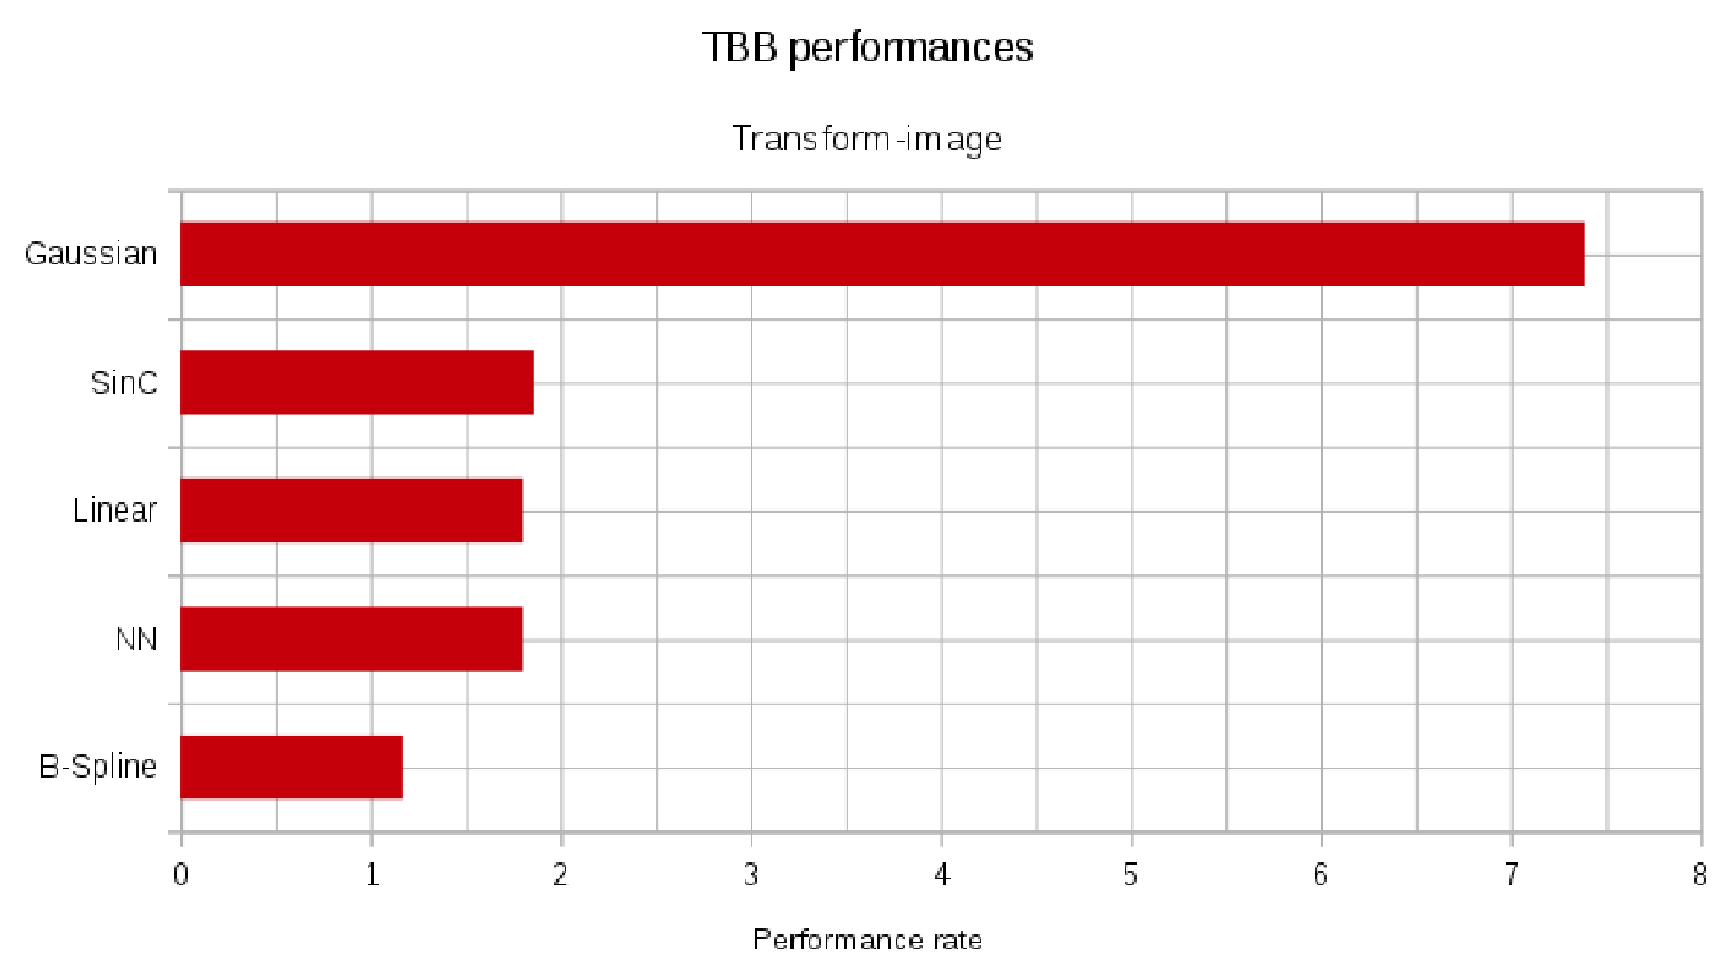
\includegraphics[width=10cm]{figures/performances_tbb_transform_image.eps}	
	\caption{Taux d'amélioration de "transform-image" avec TBB en fonction des interpolations}
	\label{Taux d'amélioration de "transform-image" avec TBB en fonction des interpolations}
\end{wrapfigure}

Dans un premier temps, on étudie la quantité d'intructions fournies par le programme. Par conséquent, plus le nombre d'instructions est grand, plus l'exécution sera longue.\newline  
- L'interpolation Gaussienne révèle des performances quasiment 8 fois supérieures lorsque le programme est parrallélisé (quasiment idéal pour une parrallélisation sur 8 CPUs).\newline
- L'interpolation en sinus cardinal, bien que moins coûteuse en ressources, ne révèle pas une parrallélisation aussi performante (performances environ doublées), de même que pour les autres interpolations .
\newline

\newpage
\underline{Anlyse des fuites de caches:} \newline\newline  
Un autre aspect important a prendre en compte lors du profilage est la quantité de fuites de caches. Ceci permet d'avoir des renseignements sur la gestion de la mémoire. Comme on peut le voir ci-dessous, les fuites de caches sont tellement minimes qu'elles sont indécelables sur la totalité des instructions (de l'ordre de quelques milliers de fuites sur plusieurs milliards d'instructions). \newline
En revanche, la présence de "mispredictions" c'est à dire des branches du code qui n'ont pas été exploré (à cause d'une condition, par exemple). Cet aspect n'a pas de rapport direct avec la mémoire, mais est un élément principal à prendre en compte dans le pipeline du programme.
\begin{figure}[h!]
	\begin{center}
		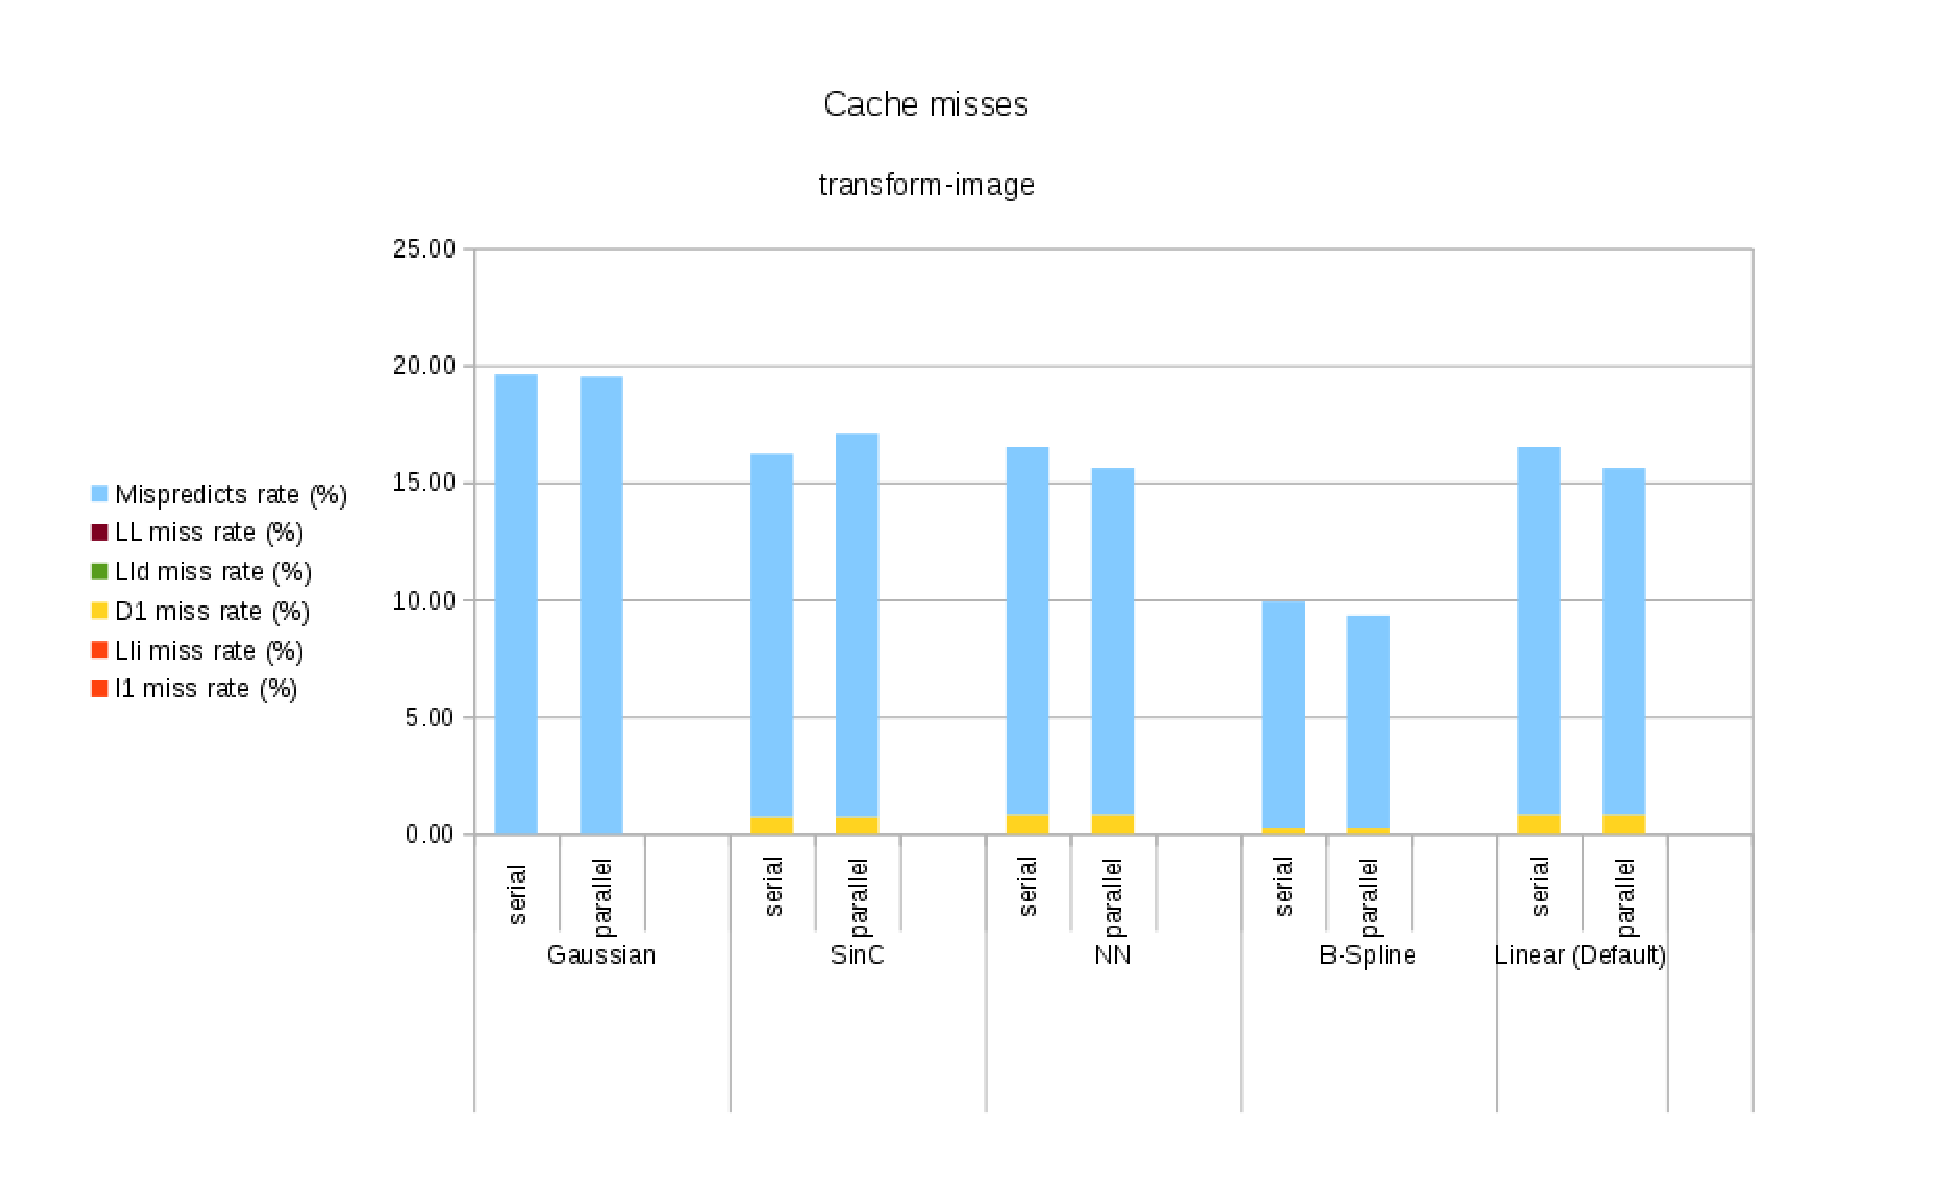
\includegraphics[height=8cm]{figures/cache_misses_transform_image.eps}
		\caption{Taux de fuites de caches et de fausses prédictions}
		\label{Taux de fuites de caches et de fausses prédictions}
	\end{center}
\end{figure}
\newline\newline 
{$\bullet$} \textit{Downsample-image} \newline
\begin{wrapfigure}[7]{r}{8cm}
	
	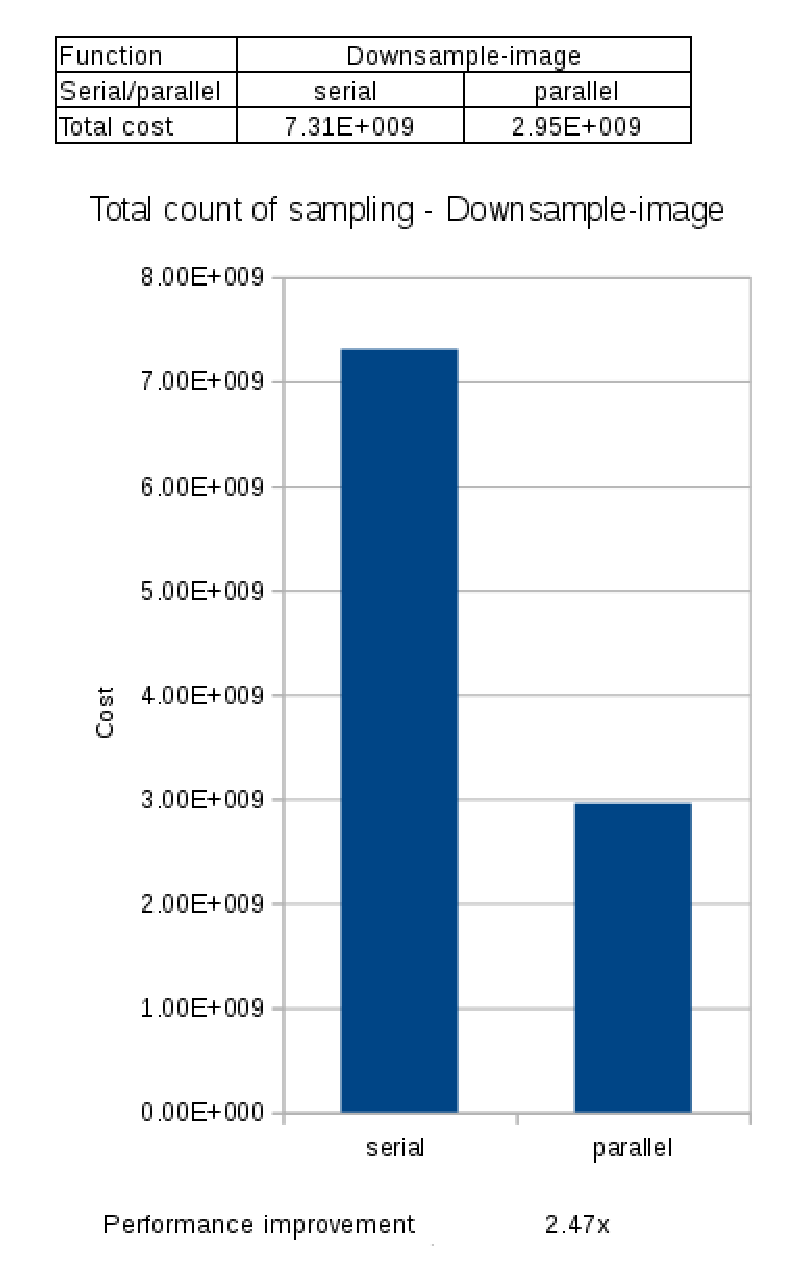
\includegraphics[height=8cm]{figures/downsample_image_costs.eps}
	\caption{Taux d'amélioration de "downsample-image" avec TBB}
	\label{Taux d'amélioration de "downsample-image" avec TBB}
\end{wrapfigure}
La fonction downsample a pour but de sous-échantilloner une image avec un filtre itératif avec la méthode de la pyramide Gaussienne. C'est-à-dire que la taille de l'image est réduite par un processus mathématique défini.\newline
On peut voir ci-contre qu'activer TBB pour cette fonction augmente les performances d'un ratio de 2,47. Il y a environ 4 milliards d'instructions en moins dans le thread principal lorsque le programme est exécuté de manière parallèle. \newline\newline\newline\newline\newline\newline\newline\newline\newline\newline\newline\newline\newline\newline\newline\newline



{$\bullet$} \textit{Smooth-image} \newline
\begin{wrapfigure}[7]{r}{8cm}
	
	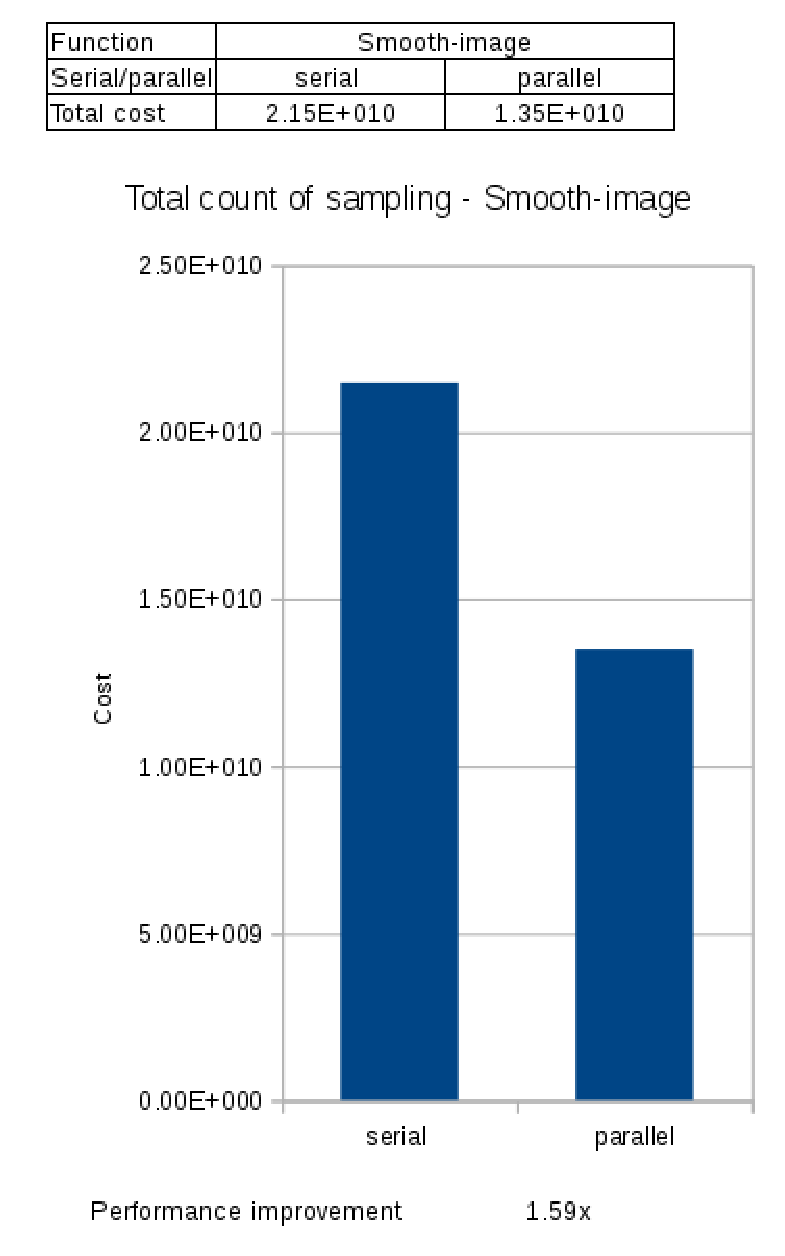
\includegraphics[height=8cm]{figures/smooth_image_costs.eps}
	\caption{Taux d'amélioration de "smooth-image" avec TBB}
	\label{Taux d'amélioration de "smotth-image" avec TBB}
\end{wrapfigure}
La fonction smooth a pour but de flouter une image passée en entrée. \newline
On peut voir ci-contre qu'activer TBB pour cette fonction augmente les performances d'un ratio de 1,59. Il y a environ 8 milliards d'instructions en moins dans le thread principal lorsque le programme est exécuté de manière parallèle.
\chapter*{Bazar}
- Inscription au RSE (Research Sofware Engineering) pour le 26/05/2016


\end{document}